\documentclass{article}

% Language setting
% Replace `english' with e.g. `spanish' to change the document language
\usepackage[english]{babel}

% Set page size and margins
% Replace `letterpaper' with `a4paper' for UK/EU standard size
\usepackage[letterpaper,top=2cm,bottom=2cm,left=3cm,right=3cm,marginparwidth=1.75cm]{geometry}

\newcommand{\mat}[1]{\mathbf{#1}}
% ----- vectors ----------------------------
%
\newcommand{\va}{\vec a}
\newcommand{\vb}{\vec b}
\newcommand{\vc}{\vec c}
\newcommand{\vd}{\vec d}
\newcommand{\ve}{\vec e}
\newcommand{\vf}{\vec f}
\newcommand{\vg}{\vec g}
\newcommand{\vh}{\vec h}
\newcommand{\vi}{\vec i}
\newcommand{\vj}{\vec j}
\newcommand{\vk}{\vec k}
\newcommand{\vl}{\vec l}
\newcommand{\vm}{\vec m}
\newcommand{\vn}{\vec n}
\newcommand{\vo}{\vec o}
\newcommand{\vp}{\vec p}
\newcommand{\vq}{\vec q}
\newcommand{\vr}{\vec r}
\newcommand{\vs}{\vec s}
\newcommand{\vt}{\vec t}
\newcommand{\vu}{\vec u}
\newcommand{\vv}{\vec v}
\newcommand{\vw}{\vec w}
\newcommand{\vx}{\vec x}
\newcommand{\vy}{\vec y}
\newcommand{\vz}{\vec z}
\newcommand{\vnull}{\vec 0}

% ----- matrices
%
%  Syntax: \M<Gro{\ss}buchstabe> bzw. \Mnull
%
\newcommand{\MA}{\mat{A}}
\newcommand{\MB}{\mat{B}}
\newcommand{\MC}{\mat{C}}
\newcommand{\MD}{\mat{D}}
\newcommand{\ME}{\mat{E}}
\newcommand{\MF}{\mat{F}}
\newcommand{\MG}{\mat{G}}
\newcommand{\MH}{\mat{H}}
\newcommand{\MI}{\mat{I}}
\newcommand{\MJ}{\mat{J}}
\newcommand{\MK}{\mat{K}}
\newcommand{\ML}{\mat{L}}
\newcommand{\MM}{\mat{M}}
\newcommand{\MN}{\mat{N}}
\newcommand{\MO}{\mat{O}}
\newcommand{\MP}{\mat{P}}
\newcommand{\MQ}{\mat{Q}}
\newcommand{\MR}{\mat{R}}
\newcommand{\MS}{\mat{S}}
\newcommand{\MT}{\mat{T}}
\newcommand{\MU}{\mat{U}}
\newcommand{\MV}{\mat{V}}
\newcommand{\MW}{\mat{W}}
\newcommand{\MX}{\mat{X}}
\newcommand{\MY}{\mat{Y}}
\newcommand{\MZ}{\mat{Z}}
\newcommand{\Mnull}{\mat{0}}
% Useful packages
\usepackage{amsmath}
\usepackage{graphicx}
\usepackage[colorlinks=true, allcolors=blue]{hyperref}
\usepackage{cleveref}
\usepackage[most]{tcolorbox}


\title{Rotation matrix clarification}
\author{Mauhing Yip}

\begin{document}
\maketitle

\section{Derivation of rotation matrix}
Let $\vk_1$, $\vk_2$ and $\vk_3$ be a unit vector\footnote{In this document, we use the term vector without properly define vector space.} and orthogonal to each others. We call them \textbf{basis vectors} in frame $K$. Similarly, $\vg_1$, $\vg_2$, $\vg_3$ for frame $G$.
Given a vector $\vec{r}$ and we expressed it into the frame $K$ and $G$ (they share same origo) in the following:
\begin{align*}
    \vec{r} 
    &=
    [\vec{k}_1, \vec{k}_2, \vec{k}_3]
    \begin{bmatrix}
      r^k_1 \\
      r^k_2 \\
      r^k_3
    \end{bmatrix}
    =
    [\vec{g}_1, \vec{g}_2, \vec{g}_3]
    \begin{bmatrix}
      r^g_1 \\
      r^g_2 \\
      r^g_3 
    \end{bmatrix}
    \\
    &= r^k_1\vec{k}_1 + r^k_2\vec{k}_2 + r^k_3\vec{k}_3
    = r^g_1\vec{g}_1 + r^g_2\vec{g}_2 + r^g_3\vec{g}_3.
\end{align*}
We want to find the relation between $[r^k_1, r^k_2, r^k_3]^T$ and $[r^g_1, r^g_2, r^g_3]^T$. We proceed as follows:
\begin{align*}
    [\vec{k}_1, \vec{k}_2, \vec{k}_3]
    \begin{bmatrix}
      r^k_1 \\ r^k_2 \\ r^k_3
    \end{bmatrix}
    &=
    [\vec{g}_1, \vec{g}_2, \vec{g}_3]
    \begin{bmatrix} 
      r^g_1 \\ r^g_2 \\ r^g_3 
    \end{bmatrix}
    \\
    \begin{bmatrix}
      \vec{k}_1 \\ \vec{k}_2 \\ \vec{k}_3
    \end{bmatrix}
    \cdot
    [\vec{k}_1, \vec{k}_2, \vec{k}_3]
    \begin{bmatrix}
      r^k_1 \\ r^k_2 \\ r^k_3
    \end{bmatrix}
    &=
    \begin{bmatrix}
      \vec{k}_1 \\ \vec{k}_2 \\ \vec{k}_3
    \end{bmatrix}
    \cdot
    [\vec{g}_1, \vec{g}_2, \vec{g}_3]
    \begin{bmatrix}
      r^g_1 \\ r^g_2 \\ r^g_3
    \end{bmatrix}
    \\
    \begin{bmatrix}
      r^k_1 \\ r^k_2 \\ r^k_3
    \end{bmatrix}
    &= \mathbf{R}_{K,G}
    \begin{bmatrix}
      r^g_1 \\ r^g_2 \\ r^g_3
    \end{bmatrix},
\end{align*}
where $\cdot$ is the dot product between vectors, and the definition of rotation $\MR_{K,G}$
\begin{align}
    \MR_{K,G} 
    &=
    \begin{bmatrix}
      \vec{k}_1 \\ \vec{k}_2 \\ \vec{k}_3
    \end{bmatrix}
    \cdot
    [\vec{g}_1, \vec{g}_2, \vec{g}_3]\\
    &=
    \begin{bmatrix}
      \vec{k}_1 \cdot \vec{g}_1 & \vec{k}_1 \cdot \vec{g}_2 & \vec{k}_1 \cdot \vec{g}_3 \\
      \vec{k}_2 \cdot \vec{g}_1 & \vec{k}_2 \cdot \vec{g}_2 & \vec{k}_2 \cdot \vec{g}_3 \\
      \vec{k}_3 \cdot \vec{g}_1 & \vec{k}_3 \cdot \vec{g}_2 & \vec{k}_3 \cdot \vec{g}_3
    \end{bmatrix}.
    \label{eq:matrix_of_dotproduct}
\end{align}
From above equation, we can see the rotation matrix is actually specified by inner product between two basis vectors and not coordinate frames are involved. 

\paragraph{To derive $\MR_{\vec{k}_1}$,} we rotate the frame $K$ w.r.t vector $\vec{k}_1$ with $\theta$ degree and denote the rotated frame as $G$. Again,  positive rotation follows the right-hand rule. \cref{fig:first_rotation} depicts the rotation, we can see that:
\begin{align*}
    \vec{k}_1\cdot\vec{g}_1 &= 1 \\
    \vec{k}_1\cdot\vec{g}_2 = \vec{k}_1\cdot\vec{g}_3 = \vec{k}_2\cdot\vec{g}_1 = \vec{k}_3\cdot\vec{g}_1 &= 0 \\
    \vec{k}_2\cdot\vec{g}_2 = \vec{k}_3\cdot\vec{g}_3 &=\cos{(\theta)}\\
    \vec{k}_3\cdot\vec{g}_2 &=\cos{(\frac{\pi}{2} + \theta)} \\
    \vec{k}_2\cdot\vec{g}_3 &=\cos{(\frac{\pi}{2} - \theta)}.
\end{align*}
Since $\cos{(\frac{\pi}{2} - \theta)} = \sin{(\theta)}$, and $\cos{(\frac{\pi}{2} + \theta)} = -\sin{(\theta)}$, the rotation matrix $\MR_{\vec{k}_1}$ in \cref{eq:matrix_of_dotproduct} becomes:
\begin{equation*}
    \begin{bmatrix}
      1 & 0 & 0 \\
      0 & \cos{\theta} & -\sin{\theta} \\
      0 & \sin{\theta} & \cos{\theta}
    \end{bmatrix}.
\end{equation*}

\begin{figure}[h]
    \centering
    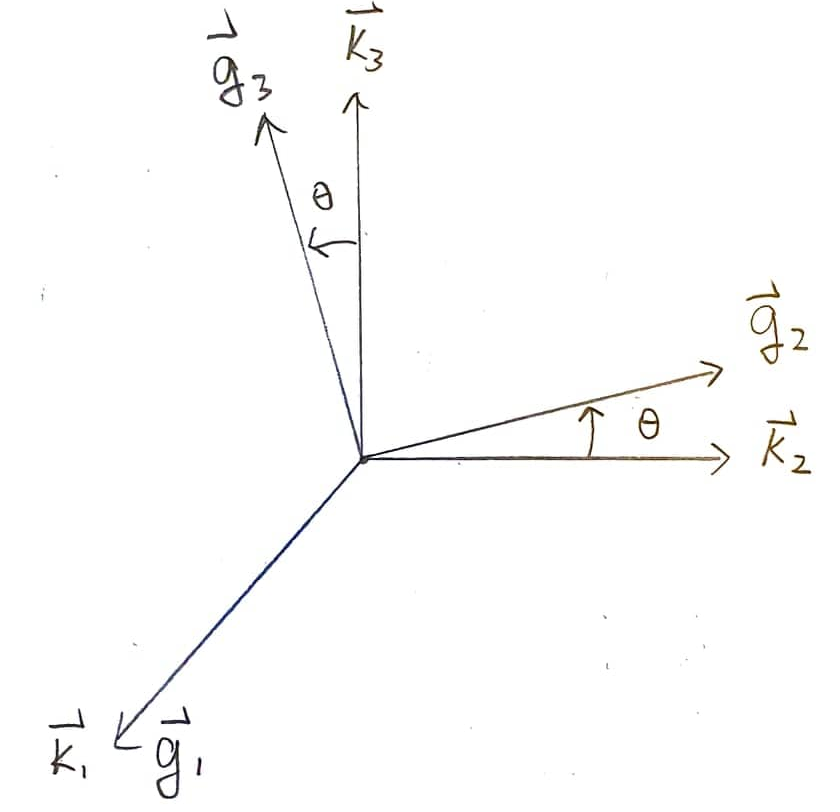
\includegraphics[width=0.4\textwidth]{Figures/UWS-rotation-first.png}
    \caption{Rotation w.r.t $\vec{k}_1$}
    \label{fig:first_rotation}
\end{figure}

\paragraph{To derive $\MR_{\vec{k}_2}$,} we rotate the frame $K$ w.r.t vector $\vec{k}_2$ with $\psi$ degree and denote the rotated frame as $G$. The positive rotation follows the right-hand rule. \cref{fig:second_rotation} depicts the rotation, we can see that:
\begin{align*}
    \vec{k}_2\cdot\vec{g}_2 &=1 \\
    \vec{k}_1\cdot\vec{g}_2 = \vec{k}_3\cdot\vec{g}_2 = \vec{k}_2\cdot\vec{g}_1 = \vec{k}_2\cdot\vec{g}_3 &= 0 \\
    \vec{k}_1\cdot\vec{g}_1 = \vec{k}_3\cdot\vec{g}_3 &=\cos{(\psi)}\\
    \vec{k}_3\cdot\vec{g}_1 &=\cos{(\frac{\pi}{2} + \psi)} \\
    \vec{k}_1\cdot\vec{g}_3 &=\cos{(\frac{\pi}{2} - \psi)}.
\end{align*}
Since $\cos{(\frac{\pi}{2} - \psi)} = \sin{(\psi)}$, and $\cos{(\frac{\pi}{2} + \psi)} = -\sin{(\psi)}$, the rotation matrix $\MR_{\vec{k}_2}$ in \cref{eq:matrix_of_dotproduct} becomes:
\begin{equation*}
    \begin{bmatrix}
      \cos{\theta} & 0 & \sin{\psi} \\
      0 & 1 & 0 \\
      -\sin{\theta} & 0 & \cos{\psi}
    \end{bmatrix}.
\end{equation*}

\begin{figure}[h]
    \centering
    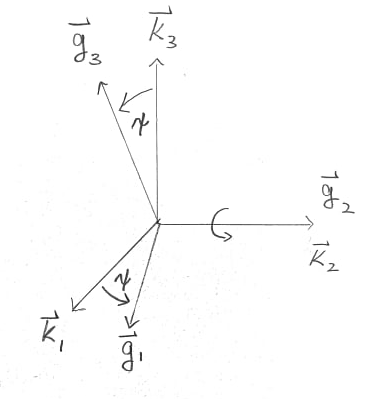
\includegraphics[width=0.4\textwidth]{Figures/UWS-rotation-second.png}
    \caption{Rotation w.r.t $\vec{k}_2$}
    \label{fig:second_rotation}
\end{figure}

\paragraph{To derive $\MR_{\vec{k}_3}$,} we rotate the frame $K$ w.r.t vector $\vec{k}_3$ with $\phi$ degree and denote the rotated frame as $G$. Again, positive rotation follows the right-hand rule. \cref{fig:third_rotation} depicts the rotation, we can see that:
\begin{align*}
    \vec{k}_3\cdot\vec{g}_3 &=1 \\
    \vec{k}_3\cdot\vec{g}_1 = \vec{k}_3\cdot\vec{g}_2 = \vec{k}_2\cdot\vec{g}_1 = \vec{k}_1\cdot\vec{g}_3 &= 0 \\
    \vec{k}_1\cdot\vec{g}_1 = \vec{k}_2\cdot\vec{g}_2 &=\cos{(\phi)}\\
    \vec{k}_1\cdot\vec{g}_2 &=\cos{(\frac{\pi}{2} + \phi)} \\
    \vec{k}_2\cdot\vec{g}_1 &=\cos{(\frac{\pi}{2} - \phi)}.
\end{align*}
Since $\cos{(\frac{\pi}{2} - \phi)} = \sin{(\phi)}$, and $\cos{(\frac{\pi}{2} + \phi)} = -\sin{(\phi)}$, the rotation matrix $\MR_{\vec{k}_3}$ in \cref{eq:matrix_of_dotproduct} becomes:
\begin{equation*}
    \begin{bmatrix}
      \cos{\phi} & -\sin{\phi} & 0 \\
      \sin{\phi} & \cos{\phi} & 0 \\
      0 & 0 & 1
    \end{bmatrix}.
\end{equation*}

\begin{figure}[h]
    \centering
    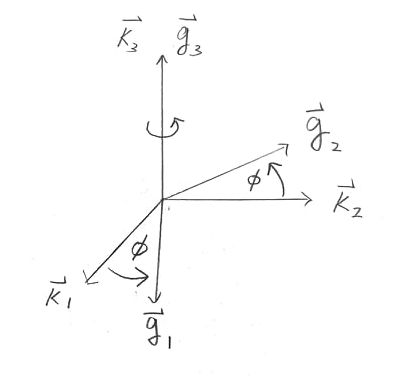
\includegraphics[width=0.4\textwidth]{Figures/UWS-rotation-third.png}
    \caption{Rotation w.r.t $\vec{k}_3$}
    \label{fig:third_rotation}
\end{figure}


\begin{equation*}
    \mathbf{R}_{\vec{k}_1} (\theta) = 
    \begin{bmatrix}  
  1 & 0 & 0 \\  
  0 & \cos{\theta} & -\sin{\theta} \\
  0 & \sin{\theta} & \cos{\theta}   
\end{bmatrix} ,
\label{eq:pitch}
\end{equation*} 
\begin{equation*}
    \mathbf{R}_{\vec{k}_2} (\psi) = \begin{bmatrix}  
  \cos{\psi} & 0 & \sin{\psi} \\  
  0 & 1 & 0 \\
  -\sin{\psi} & 0 & \cos{\psi}   
\end{bmatrix}, 
\end{equation*}
\begin{equation*}
    \mathbf{R}_{\vec{k}_3} (\phi) = \begin{bmatrix} 
  \cos{\phi} & -\sin{\phi} & 0 \\
  \sin{\phi} & \cos{\phi} & 0 \\
  0 & 0 & 1
\end{bmatrix}. 
\end{equation*}

\section{Intrinsic (mobile frame) rotation and extrinsic (fixed frame) rotation}
The statement "We first rotate around $\vk_1$, then rotate around $\vk_2$" can means two things and it is ambiguous. 
If we first rotate around $\vk_1$, then $\vk_2$ and $\vk_3$ will change. Then, by rotating around $\vk_2$, it can mean rotate around $vk_2$ before it gets changed (extrinsic rotation) or rotate around $\vk_2$ after it gets changed (intrinsic rotation). In this doc, we only use extrinsic rotation. To interactively see the difference between intrinsic and extrinsic rotation, you check the website: \url{https://www.mecademic.com/en/how-is-orientation-in-space-represented-with-euler-angles}.

\section{Interpretation of rotation matrix}
The complete consecutive rotation is the following
\begin{equation}
\MR_{K,G} (\theta, \psi, \phi) = R_{\vec{k}_3}(\phi)R_{\vec{k}_2}(\psi)R_{\vec{k}_1}(\theta).
\label{eq:rotation_compose}
\end{equation}
Below shows what we can do with the rotation matrix $\MR_{K,G}$. The rotation matrix $\MR_{K,G}$ transfer the basis vectors of frame $K$ to the basis vectors of frame $G$ in the following way.
\begin{equation}
    [\vec{g}_1, \vec{g}_2, \vec{g}_3] = [\vec{k}_1, \vec{k}_2, \vec{k}_3]
    \begin{bmatrix}
      r_{1,1} & r_{1,2} & r_{1,3} \\
      r_{2,1} & r_{2,2} & r_{2,3} \\
      r_{3,1} & r_{3,2} & r_{3,3}
    \end{bmatrix},
    \quad \textrm{where} \quad
    \begin{bmatrix}
      r_{1,1} & r_{1,2} & r_{1,3} \\
      r_{2,1} & r_{2,2} & r_{2,3} \\
      r_{3,1} & r_{3,2} & r_{3,3}
    \end{bmatrix}
    := \MR_{K,G}.
    \label{eq:vector_transformation}
\end{equation}
We can write them even more explicitly in the following way:
\begin{equation*}
    \begin{array}{l} 
      \vec{g}_1= r_{1,1}\vec{k}_1 + r_{2,1}\vec{k}_2 + r_{3,1}\vec{k}_3\\
      \vec{g}_2= r_{1,2}\vec{k}_1 + r_{2,2}\vec{k}_2 + r_{3,2}\vec{k}_3\\
      \vec{g}_3= r_{1,3}\vec{k}_1 + r_{2,3}\vec{k}_2 + r_{3,3}\vec{k}_3\\
    \end{array},
\end{equation*}
which shows the direct relation basis vectors of frame $K$ and basis vectors of frame $G$. Beware that the square bracket $[\vec{k}_1, \vec{k}_2, \vec{k}_3]$ is a row-array of vectors, not vector's components. We refer \cref{eq:vector_transformation} as \textbf{basis vectors transformation} and no coordinates are involved.

Now, we have point $p$, and it is expressed in the basis vectors of $G$ with a vector $\vec{p} = p^g_1\vec{g}_1 + p^g_2\vec{g}_2 + p^g_3\vec{g}_3$. If we multiply the column array $[p^g_1, p^g_2, p^g_3]^T$ on both side of equation \ref{eq:vector_transformation} from the right. We have:
\begin{equation}
    [\vec{g}_1, \vec{g}_2, \vec{g}_3] \begin{bmatrix}
      p^g_1 \\
      p^g_2\\
      p^g_3
    \end{bmatrix}
    = [\vec{k}_1, \vec{k}_2, \vec{k}_3]
    \begin{bmatrix}
      r_{1,1} & r_{1,2} & r_{1,3} \\
      r_{2,1} & r_{2,2} & r_{2,3} \\
      r_{3,1} & r_{3,2} & r_{3,3}
    \end{bmatrix}
    \begin{bmatrix}
      p^g_1 \\
      p^g_2\\
      p^g_3
    \end{bmatrix}.
    \label{eq:change_coordinate}
\end{equation}
We obtain
\begin{equation*}
\begin{split}
\vec{p} & = (p^g_1r_{1,1} + p^g_2r_{1,2} + p^g_3r_{1,3})\vec{k}_1 \\
 & \quad + (p^g_1r_{2,1}+p^g_2r_{2,2}+p^g_3r_{2,3})\vec{k}_2 \\
 & \quad \quad + (p^g_1r_{3,1}+p^g_2r_{3,2}+p^g_3r_{3,3})\vec{k}_3 \\
 & = p^k_1\vec{k}_1 + p^k_2\vec{k}_2 + p^k_3\vec{k}_3,
\end{split}
\end{equation*}
where the vector $\vec{q}$ is expressed in the basis vectors of $K$. In another word, the vector's components are calculated in the following way: 
\begin{equation*}
\begin{bmatrix}
      p^k_1 \\
      p^k_2\\
      p^k_3
\end{bmatrix}
    =
    \begin{bmatrix}
      r_{1,1} & r_{1,2} & r_{1,3} \\
      r_{2,1} & r_{2,2} & r_{2,3} \\
      r_{3,1} & r_{3,2} & r_{3,3}
    \end{bmatrix}
    \begin{bmatrix}
      p^g_1 \\
      p^g_2\\
      p^g_3
    \end{bmatrix}.
\end{equation*}
A more compact expression can be: 
\begin{equation}
\mathbf{p}^K = \MR_{K,G} \mathbf{p}^G
    \label{eq:coordinate_transformation},
\end{equation}
where the $\mathbf{p}^K$ is the vector components of $p$ in the frame $K$, likewise for $\mathbf{p}^G$. Equation \ref{eq:coordinate_transformation} is very common in varies text book. We refer \cref{eq:coordinate_transformation} as \textbf{coordinate transformation}.

Remark: The \textbf{basis vectors transformation} (\cref{eq:vector_transformation}) is a transformation that transform from the basis vectors  $\vec{k}_1, \vec{k}_2, \vec{k}_3$ to the basis vectors $\vec{g}_1, \vec{g}_2, \vec{g}_3$. In contrary, the \textbf{coordinate transformation} (\cref{eq:coordinate_transformation}) is a transformation of changing coordinate frame of the point $p$ from frame $G$ to frame $K$. From \cref{eq:change_coordinate} and \cref{eq:vector_transformation} shows us that the rotation matrix $\MR_{K,G}$ transform the basis vectors in a way that from $K$ to $G$, but $\MR_{K,G}$ transform coordinate (vector's component) in a opposite way that from $G$ to $K$. This is well known relation in tensor calculus because vector is co-variant object and vector's components is contra-variant object.

Here, we summarize the meaning of the subscript of the rotation $\MR_{K,G}$. It can have two meaning:
\begin{tcolorbox}
\begin{enumerate}
    \item $\MR_{K,G}$ transforms the coordinate of a point \textbf{from $G$ to $K$}. (\textbf{coordinate transformation})
    \item $\MR_{K,G}$ transforms the set of basis vectors \textbf{from $K$ to $G$}. (\textbf{basis vectors transformation})
\end{enumerate}
\end{tcolorbox}
We mainly use the \textbf{coordinate transformation} to interpret the rotation matrix $\MR_{K,G}$ in this document.

%\bibliographystyle{alpha}
%\bibliography{sample}

\end{document}